
\section{Case Study}

\subsection{Scenario Generation}
As already mentioned in subsection \ref{sub:Uncertainty_Characterization}, our model has to account for variations concerning solar and wind power generation in between the clearance of the day-ahead and adjustment market, denoted by $\overline{P}^{W}$ and $\overline{P}^{S}$, and during the market horizon, denoted by ${P}^{W}$ and ${P}^{S}$, as well as the prices at the day-ahead and adjustment market, $\lambda^D$ and $\lambda^A$, and the imbalance price ratios $r^+$,$r^-$. Market prices are assumed to be independent of power generation. However, interdependencies within the sets of $\left\lbrace\overline{P}^{W},{P}^{W},\overline{P}^{S},{P}^{S}\right\rbrace$ and $\left\lbrace\lambda^D,\lambda^A,r^+,r^-\right\rbrace$ respectively can not be neglected. Without losing generality, we limit our analysis to a single time period noon - 1.00 PM. Furthermore, for simplicity, we utilise the market scenario of page 220 of \cite{Conejo10}. %but extend it by a second version where $E\left[\lambda^D-\lambda^A\right]<0$
Our goal is to model an even split between solar and wind energy on an average day concerning power generation. To do so, we analysed historical data from the 50Hertz control area in Germany  \cite{url}. The data set supplies hourly power generation from the January 1st, 2015, to October 1st, 2020. As mentioned before, solar and wind power generation is strongly dependent on the weather and exhibits strong seasonal effects. While such seasonal effects have interesting economic implications on their own, they should not drive the variance of power generation in our scenarios. In other words, making use of scenarios that best represent the market for a variety of seasons would exaggerate the spread in power generation and hence not represent the energy market at any day throughout the analysed period. Furthermore, in the data set, the average power generation from wind is 216\% higher than the solar power generation. To mitigate the skewness towards wind energy and the seasonal effects, we first normalise the average power generation of both supply streams to $5.000 MW$. Second, we subtract the 30-day moving average and reapply the overall average $\left(\sim 5.000 MW\right)$. Note that our model solar energy will nevertheless outweigh wind energy due to our focus on the 12:00 PM - 13:00 PM market horizon. To account for the negative correlation between solar and wind power generation, we fit both supply streams to ARMA models of the form $y_t = \mu + \phi \left(y_{t-1}-\mu\right)+\varepsilon_t + \theta\varepsilon_{t-1}$ and compute the variance-covariance Matrix $G$ of $\varepsilon^S$ and $\varepsilon^W$, where $\varepsilon^S$ $\left(\varepsilon^W\right)$ refers to the residual vector of the solar (wind) energy ARMA model. The stochastic processes 
for solar and wind energy supply can hence be described as follows:

\begin{align}
\overline{P}^{W}=& \mu^W+\epsilon_1^W\\
\overline{P}^{S}=& \mu^S+\epsilon_1^S\\
{P}^{S}=&\mu^S + \phi^S \left(\overline{P}^{S}-\mu^S\right)+\epsilon^S_2 + \theta^S\epsilon^S_1\\
{P}^{W}=&\mu^W + \phi^W \left(\overline{P}^{W}-\mu^W\right)+\epsilon^W_2 + \theta^W\epsilon^W_1.
\end{align}


Note again that $\varepsilon^S$ and $\varepsilon^W$ refer to the residual vectors from the fitted ARMA models while $\left(\epsilon_1^S,\epsilon_1^W\right)$ and $\left(\epsilon_2^S,\epsilon_2^W\right)$ correspond to two independent realizations of the same random variable distributed according to a multivariate normal distribution with variance-covariance matrix $G$ and mean $\overline{\varepsilon}^S$, $\overline{\varepsilon}^W$. Here, $\overline{\varepsilon}^S$ $\left(\overline{\varepsilon}^W\right)$ refers to the average of the residual vector $\varepsilon^S$ $\left(\varepsilon^W\right)$. The parameters $\phi^S$, $\phi^W$, $\theta^S$, $\theta^W$ refer to the parameter results of the fitted ARMA models and $\mu^S$ $\left(\mu^W\right)$ refers to the mean of the normalized historical data set for solar (wind) energy. For $\left(\epsilon_1^S,\epsilon_1^W\right)$ and $\left(\epsilon_2^S,\epsilon_2^W\right)$ respectively we generate $1.000$ realizations and cluster down to 4 branches based on euclidean distance, resulting in a total of 16 scenarios for power generation. Matching each power generation scenario with each of the eight price scenarios we get a total of 128 scenarios.




\subsection{Results}





Considering different values for risk aversion, we wish to compare a hybrid producer's revenue with the sum of two single energy producers' revenues, i.e.\ the sum of the revenues of a solar-only producer and a wind power only producer. Before starting with the optimisation results, we summarised the relevant power production measures in the table below. 


\begin{table}[h!]
	\centering
	\begin{threeparttable}
		\caption{Power production measures.}
		\begin{tabular}{llll}
			\toprule
			Measures & \( Mean \) & \( Variance \) & \( Standard \text{ } deviation \)  \\
			\midrule
			Solar Power    & 13407.17        &  2.88$\cdot 10^7$      &  5370.08     	    \\
			Wind Power    & 5890.41     &   7.37$\cdot 10^6$      &  2715.58          	\\
			Hybrid    &  19297.59        &  1.95 $\cdot 10^7$    & 4418.23     	\\
			\bottomrule
		\end{tabular}
		
	\end{threeparttable}
\end{table}

As expected, the mean power production for the hybrid producer sums up while the variance does not. However, the variance is significantly smaller than the sum of both power productions. Moreover, the variance of the hybrid power production is less than the single solar power production. This follows from the strong anti-correlation $ \text{cor} (P_{t\omega}^S,P_{t\omega}^W ) = -0.572 $ of wind power and solar power in our given scenarios.  





The way we modelled the problem, it was possible to simply neglect one energy source by setting the respective parameters to zero. Consequently, we could use the same model for all three producers. Apart from that, we optimised the revenue once for the situation with an adjustment market and once for the situation without an adjustment market. The results are summarised in the figures below.  

\begin{figure}[h!]
	\centering
	
	\begin{minipage}{0.95\textwidth}
		\subfloat{
			\centering
			\scalebox{0.75}{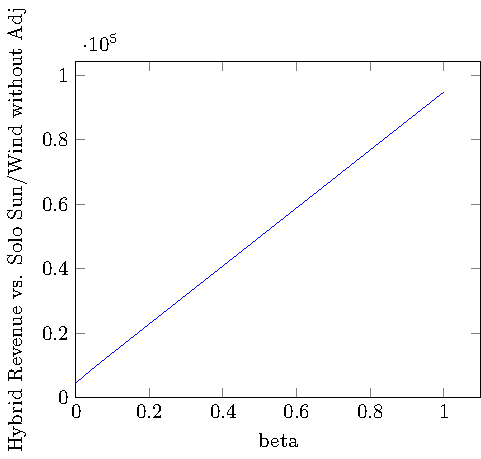
\includegraphics[]{Figures/figure2.pdf}}
		}
		\hfill
		\subfloat{
			\centering
			\scalebox{0.75}{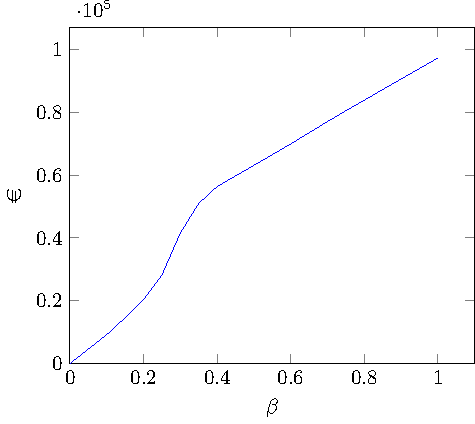
\includegraphics[]{Figures/figure.pdf}}
		}
		
		\caption{The difference of the revenues of the hybrid energy producer and the sum of both individual producers' revenue depending on the risk aversion factor $\beta$. On the left: The situation without an adjustment market. On the right: The situation with an adjustment market.  }
	\end{minipage}	
\end{figure}

We plotted the difference of the revenues of the hybrid producer and the sum of both single producers' revenues on the vertical axis. We presented the risk aversion factor $\beta$ on the horizontal axis. Overall, we see that the hybrid model is more advantageous for risk-averse producers. The more risk-averse a producer is, the more profitable it is to offer solar and wind power collectively. This is owed to having a larger mean while facing a lower variance in the collective production case. Hence, we can offer much more power for a given day-ahead price without facing more uncertainty. One striking difference is that the curve on the right starts in the origin whereas the curve on the left does not. If we have an adjustment market and are not risk-averse, it does not matter whether one producer offers both energies or two producers offer one energy each. The reason is that a risk-seeking producer offers everything on the day-ahead market and plans on buying back the deficit on the adjustment market. This is due to the producer expecting a lower price on the adjustment market $\mathbb{E}[\lambda_A]=30.45$ than on the day-ahead market $\mathbb{E}[\lambda_D]=32$ for our given data set.
On the other hand, if we do not have an adjustment market, we can exploit the anti-correlation. Thus, the variance of the produced amount of energy decreases and therefore, the hybrid producer can offer more energy for a given day-ahead price. Hence, it is more profitable to produce both collectively. 

Apart from that, we observe a linear growth behaviour in a market system without an adjustment market. When adding the adjustment market to the system, we notice a slight bump. At some value for the risk aversion factor $\beta$, the producer is not brave enough anymore to trade on arbitrage since he would face losses in specific scenarios. 

